% IEEE e-Science 2026 style: IEEE conference format (two columns, 10 pt).
\documentclass[conference]{IEEEtran}
\IEEEoverridecommandlockouts
\usepackage{cite}
\usepackage{amsmath,amssymb}
\usepackage{graphicx}
\usepackage{booktabs}
\usepackage{textcomp}
\usepackage{xcolor}
\usepackage{url}
\usepackage{tikz}
\usetikzlibrary{positioning,arrows.meta}
\usepackage[hidelinks]{hyperref}
\definecolor{aseq}{HTML}{2A78D6}
\definecolor{boxbg}{HTML}{F3F7FD}
\definecolor{ink2}{HTML}{52514E}
\newcommand{\code}[1]{{\small\texttt{#1}}}
\def\BibTeX{{\rm B\kern-.05em{\sc i\kern-.025em b}\kern-.08em T\kern-.1em\lower.7ex\hbox{E}\kern-.125em X}}

\begin{document}

\title{adaptiSeq: Parallel, Verified Retrieval of Public Sequencing Accession Lists from Unreliable Archives}

\author{\IEEEauthorblockN{Rasman Mubtasim Swargo, Nieb Hasan Neom, Md Arifuzzaman}
\IEEEauthorblockA{Missouri University of Science and Technology, Rolla, MO, USA\\
rs75c@mst.edu, nn3bd@mst.edu, marifuzzaman@mst.edu}}

\maketitle

\begin{abstract}
Reanalysis of public sequencing data starts from a list of accessions, often hundreds of runs, and every run must arrive intact before analysis can begin. We measured what this task meets on today's archives: the European Nucleotide Archive (ENA) serves each TCP connection at about 2~MB/s, its metadata service failed 3.1\% of 3,420 queries over 17 days in episodes of hours, it served corrupt copies of files that were identical on retry, and it refuses connections past a moving ceiling. Tools that fetch one file at a time over one connection take hours for a list the link could carry in minutes, and when the archive misbehaves several of them exit with status 0 while runs are missing or were silently fetched from another archive in a form that cannot be checked against ENA's checksum. We present adaptiSeq, a Python tool and library that treats the list as the unit of work: concurrent, rate-limited accession resolution; a queue of files served by a pool of workers that split each file into resumable byte ranges and keep connections busy to the last byte; a per-host guard that reads a refusal as a ceiling; checksum verification inside the pool with parallel re-fetch of bad copies; and an exit status that reflects what was delivered. It covers GSA, SRA, ENA, DDBJ and GEO, reimplements iSeq's interface, and includes several controllers for the number of files in flight. On two ENA lists (241 runs, 7.6~GB; 8 runs, 25.9~GB) on SDSC Expanse, five repetitions each, the fastest other tool that delivered every run was a median of 6.1 times slower than adaptiSeq's default and 9.8 times slower than its fixed pool on the first list. adaptiSeq never exited 0 with a run missing (0 of 20 rows), against 8 of 40 rows for iSeq, Kingfisher and fastq-dl. We also report where it does not win: a fixed pool beat the adaptive default in most repetitions, and every result depends on the state of the archive during the run.
\end{abstract}

\begin{IEEEkeywords}
sequencing data retrieval, public archives, parallel transfer, data integrity, reproducible benchmarking, ENA, SRA
\end{IEEEkeywords}

\section{Introduction}
The Sequence Read Archive (SRA)~\cite{sra}, the European Nucleotide Archive (ENA)~\cite{ena}, the DDBJ Sequence Read Archive~\cite{ddbj} and the Genome Sequence Archive (GSA)~\cite{gsa} together hold tens of millions of sequencing runs, and reanalysis of deposited runs is routine in transcriptomics, metagenomics and population genomics. The unit of work in such studies is rarely one file. A study, a meta-analysis or a pipeline starts from a project or a list of run accessions, each run resolves to one to three FASTQ files, and the job is to obtain every file, byte-identical to the archive's copy, as fast as the network allows, and to report exactly which runs could not be obtained.

Several tools address parts of this. iSeq~\cite{iseq} covers five databases with one command-line interface and verifies checksums. Kingfisher~\cite{kingfisher} tries several sources for each run, fastq-dl~\cite{fastqdl} retrieves FASTQ files from ENA or SRA, nf-core/fetchngs~\cite{fetchngs,nfcore} wraps retrieval in a Nextflow workflow, and pysradb~\cite{pysradb} exposes metadata and downloads to Python. With the exception of fetchngs and of pysradb given a thread count, these tools process the runs of a list one after another: each run is resolved, downloaded and checked before the next begins, usually over a single connection.

This is a poor match for the archives, and the mismatch is not only about speed. We monitored ENA's metadata API for 17 days and ran benchmark campaigns against ENA, NCBI and GSA for three weeks, and found five properties that a list downloader has to live with (Section~\ref{sec:problem}): throughput is limited per connection, the archive's state changes by the hour, the archive sometimes serves bad bytes, it refuses and cuts connections, and failure is easy to hide. The last one matters most to a user: when ENA's API fails, a common response is to assume the run is not in ENA and fetch the \texttt{.sra} file from NCBI instead, convert it, and report success. The converted file cannot be checked against ENA's checksum, and the exit status says nothing.

We present adaptiSeq, a Python reimplementation and extension of iSeq built for accession lists. It keeps iSeq's database coverage, command-line options and integrity checks, and changes how and when the bytes arrive. This paper makes the following contributions.
\begin{itemize}
\item A measurement of what public archives do to a list downloader (per-connection rates, API failure episodes, corrupt copies, connection ceilings), from monitoring and six benchmark campaigns on SDSC Expanse.
\item A design that answers each of these properties: concurrent rate-limited resolution, a segmented, resumable transfer engine ported from FastBioDL~\cite{fastbiodl} and extended, a per-host connection guard, checksum verification inside the worker pool, and an exit status that matches what was delivered. The tool also includes five controllers for the number of concurrent files, and a Python API.
\item An evaluation against iSeq, Kingfisher and fastq-dl on two ENA lists, five repetitions each, that scores a run as complete only if an independent verifier finds every file matching ENA's checksum, whatever the tool's exit status, together with an account of where the design does not win.
\end{itemize}

\section{Related Work}
\textbf{Retrieval tools.} The SRA Toolkit's \texttt{prefetch} is the standard acquisition path and resumes interrupted downloads; \texttt{fasterq-dump} converts to FASTQ. pysradb~\cite{pysradb} and ffq simplify the metadata layer. iSeq~\cite{iseq}, Kingfisher~\cite{kingfisher}, fastq-dl~\cite{fastqdl} and fetchngs~\cite{fetchngs} automate acquisition from several backends. Table~\ref{tab:feat} compares them on the properties relevant here, read from each tool's help output, source and documentation. adaptiSeq adds concurrency across runs and rate-limited parallel resolution to iSeq's feature set, and keeps iSeq's resume, merge and five-database coverage.

\textbf{Transfer systems.} Large scientific data movement has been studied outside genomics. Globus, GridFTP, FDT and mdtmFTP use parallel streams, managed endpoints and striping, but need suitable endpoints; public genomic downloads use ordinary client-side HTTP(S) or FTP, where only one end is under the user's control. aria2c supports segmented byte-range retrieval with user-selected connection counts. FastBioDL~\cite{fastbiodl} showed that tuning the worker count online from measured throughput helps for large SRA objects. adaptiSeq builds on that engine and is concerned with the list-level problem around it: resolution, completeness, verification and failure reporting.

\begin{table}[t]
\caption{Feature comparison at the versions benchmarked (read from each tool's help output, source and documentation).}\label{tab:feat}
\centering\scriptsize\setlength{\tabcolsep}{1.6pt}
\resizebox{\columnwidth}{!}{\begin{tabular}{@{}lcccccc@{}}
\toprule
 & \rotatebox{90}{adaptiSeq 0.1.12} & \rotatebox{90}{iSeq 1.9.9} & \rotatebox{90}{Kingfisher 0.5.0} & \rotatebox{90}{fastq-dl 4.0.1} & \rotatebox{90}{fetchngs 1.13.0} & \rotatebox{90}{pysradb 2.5.1}\\
\midrule
List in one call & \checkmark & \checkmark & \checkmark & -- & \checkmark & project\\
Several runs at once & \checkmark & -- & -- & -- & \checkmark & \checkmark\\
Rate-limited parallel resolution & \checkmark & -- & -- & -- & no cap & --\\
MD5 check & \checkmark & \checkmark & optional & \checkmark & \checkmark & --\\
Resume partial file & \checkmark & \checkmark & -- & -- & per task & \checkmark\\
Merge runs & \checkmark & \checkmark & -- & \checkmark & -- & --\\
Python API & \checkmark & -- & \checkmark & -- & -- & \checkmark\\
GSA & \checkmark & \checkmark & exper. & -- & -- & --\\
GEO & \checkmark & \checkmark & -- & -- & \checkmark & \checkmark\\
Installation & pip & conda & pip, conda & pip, conda & Nextflow & pip, conda\\
\bottomrule
\end{tabular}}
\end{table}

\section{The Problem: What the Archives Do}\label{sec:problem}
All measurements here come from SDSC Expanse compute nodes (AMD EPYC 7742, 2$\times$64 cores, node-local NVMe) reaching the archives over the public internet, which we neither controlled nor shaped. We use two lists. D1 is BioProject PRJNA916347: 241 runs, 321 files, 7.6~GB (mean 24~MB per file; 40 runs have three FASTQ files), where per-file overhead is a large share of the work. D2 is eight runs of PRJNA762469: 16 files, 25.9~GB (1.4--1.9~GB per file), where there are too few files to fill the link one file per connection.

\textbf{P1: throughput is per connection.} ENA served each connection at a median of 2.0~MB/s (38 probes of 1, 8 and 20 parallel HTTPS range requests, range 0.5--7.2~MB/s), and the aggregate grew almost linearly with the number of connections: the median job got 36.2~MB/s with 20, 18.4 times its single-connection rate (Fig.~\ref{fig:probe}). A tool that uses one connection per file leaves most of the path idle, whatever the network.

\begin{figure}[t]
\centering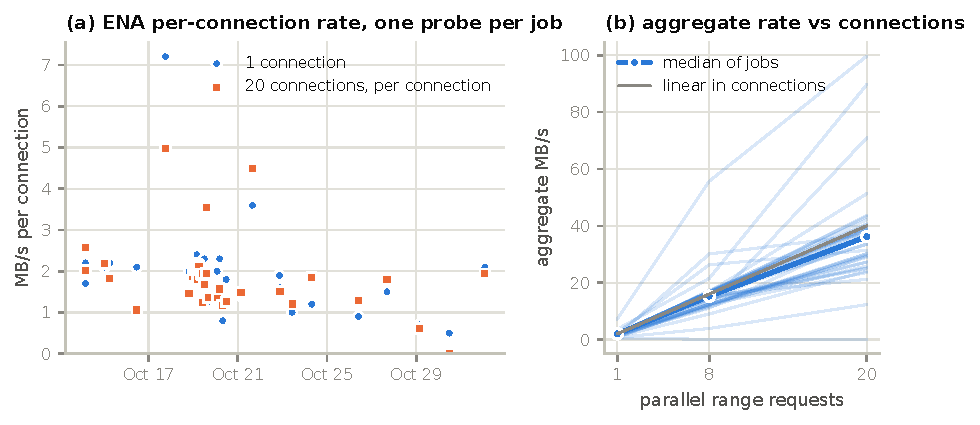
\includegraphics[width=\columnwidth]{figs/link_probe.pdf}
\caption{ENA's per-connection rate. Each benchmark job began with a 20-second probe of 1, 8 and 20 parallel HTTPS range requests to one ENA file. (a) Per-connection rate by date. (b) Aggregate rate against connections, one line per job.}\label{fig:probe}
\end{figure}

\textbf{P2: the archive's state changes by the hour.} The per-connection rate varied more than tenfold between days. ENA's metadata service was less stable still. We queried its \texttt{filereport} API every five minutes for 17 days (3,420 queries): 107 (3.1\%) failed with HTTP 500 (80) or no answer within 60~s (27), 212 more took over 10~s, and 7 came back as HTTP 200 with no rows for a run that exists. Failures cluster into episodes of hours; during one, every tool that relies on the API is affected, and a benchmark arm that happens to run then measures the episode, not the tool (Fig.~\ref{fig:portal}).

\begin{figure}[t]
\centering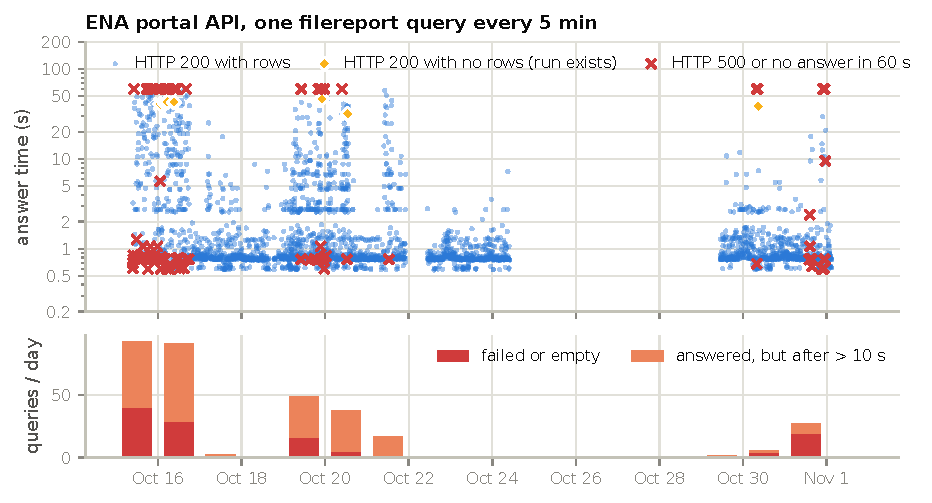
\includegraphics[width=\columnwidth]{figs/portal.pdf}
\caption{ENA's portal API over 17 days. Top: answer time of each query (log scale); crosses are HTTP 500 or no answer in 60~s, diamonds are HTTP 200 with no rows for a run that is in ENA. Bottom: failed or empty and slow answers per day.}\label{fig:portal}
\end{figure}

\textbf{P3: the archive sometimes serves bad bytes.} We counted 178 MD5 mismatches in the logs of 96 benchmark rows of the two main campaigns, in 44 of the rows. They hit every tool, landed on different files in different arms of the same hour, and a plain \texttt{curl} over FTP produced a file of exactly the right length with the wrong checksum. The same file can stay bad for days: one run of D1 failed three times in both adaptiSeq arms on Oct 27--29 after every arm had fetched it cleanly on Oct 26. A downloader cannot prevent this; it can detect it and fetch again.

\textbf{P4: the archive refuses and cuts connections.} ENA accepted about 25 simultaneous connections from one client and refused further connects; the ceiling moved (25 on some days, 50 on others). It also ended some responses short of their \texttt{Content-Length}, answered some range requests with 403 or 416, and reset FTP data connections under load. GSA cut streams at any load. A client that reads each of these as ``the server is overloaded'' backs off to a few connections and stays there.

\textbf{P5: failure is easy to hide.} When ENA's API fails, the common response is to fetch the run's \texttt{.sra} file from NCBI and convert it, which cannot be checked against ENA's MD5, and still report success. Other tools stop at the first corrupt file, or give up on a run after retries, and still exit 0. A user who trusts the exit status gets an incomplete or unverifiable data set without being told.

\section{Design}\label{sec:design}
adaptiSeq (0.1.12 throughout) keeps iSeq's command line and its accession, metadata, integrity and merge behaviour~\cite{iseq}, reimplemented in Python, and replaces the transfer path. All sequence bytes pass through one download seam, so the scheduler and engine change how and when bytes arrive, never which bytes. Fig.~\ref{fig:arch} shows the path of a list.

\begin{figure*}[t]
\centering
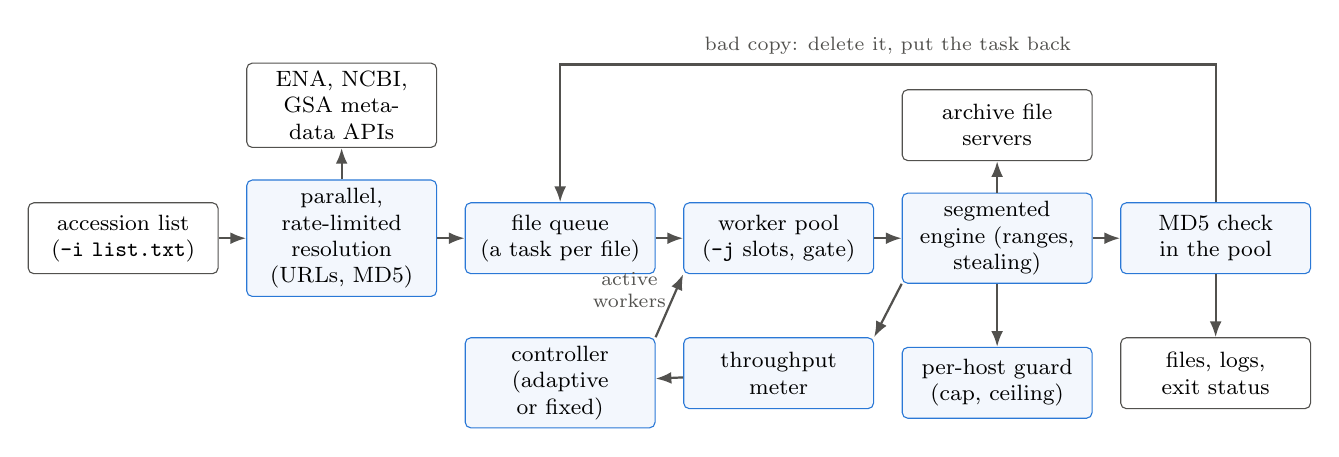
\begin{tikzpicture}[
  node distance=4mm and 3.5mm,
  box/.style={draw=aseq, fill=boxbg, rounded corners=2pt, align=center, font=\footnotesize, inner sep=3pt, minimum height=9mm, text width=2.2cm},
  ext/.style={draw=ink2, fill=white, rounded corners=2pt, align=center, font=\footnotesize, inner sep=3pt, minimum height=9mm, text width=2.2cm},
  arr/.style={-{Latex[length=2mm]}, draw=ink2, thick},
  lab/.style={font=\scriptsize, text=ink2, align=center}]
\node[ext] (list) {accession list\\(\texttt{-i list.txt})};
\node[box, right=of list] (res) {parallel, rate-limited resolution (URLs, MD5)};
\node[box, right=of res] (queue) {file queue\\(a task per file)};
\node[box, right=of queue] (pool) {worker pool\\(\texttt{-j} slots, gate)};
\node[box, right=of pool] (eng) {segmented engine (ranges, stealing)};
\node[box, right=of eng] (ver) {MD5 check in the pool};
\node[ext, above=of res] (api) {ENA, NCBI, GSA metadata APIs};
\node[ext, above=of eng] (arch) {archive file servers};
\node[box, below=8mm of queue] (ctrl) {controller (adaptive or fixed)};
\node[box, below=8mm of pool] (meter) {throughput meter};
\node[box, below=8mm of eng] (guard) {per-host guard (cap, ceiling)};
\node[ext, below=8mm of ver] (out) {files, logs, exit status};
\draw[arr] (list) -- (res); \draw[arr] (res) -- (api); \draw[arr] (res) -- (queue);
\draw[arr] (queue) -- (pool); \draw[arr] (pool) -- (eng); \draw[arr] (eng) -- (arch);
\draw[arr] (eng) -- (ver); \draw[arr] (ver) -- (out); \draw[arr] (eng) -- (guard);
\draw[arr] (eng.south west) -- (meter.north east); \draw[arr] (meter) -- (ctrl);
\draw[arr] (ctrl.north east) -- node[lab, left, pos=0.75]{active\\workers} (pool.south west);
\draw[arr] (ver.north) |- ++(0,1.75) -| node[lab, above, pos=0.25]{bad copy: delete it, put the task back} (queue.north);
\end{tikzpicture}
\caption{The path of an accession list through adaptiSeq. Resolution runs in parallel under per-archive request limits. Each file becomes a task; workers take tasks, the engine splits each file into byte ranges on several connections, a per-host guard bounds the connections and reacts to refusals, and each finished file is MD5-checked inside the pool. A bad copy goes back to the queue.}\label{fig:arch}
\end{figure*}

\subsection{Resolution under an unreliable API}
Accessions are resolved concurrently (\texttt{--meta-jobs}, default 3) under per-endpoint token buckets: 8 requests/s for ENA, 5 for GSA, 3 for NCBI (10 with an API key). Resolution yields each file's URL, size and the archive's MD5. ENA's API fails in ways that look like an answer (P2): HTTP 500 with an HTML page, an in-band error line under HTTP 200, an empty body, or an empty table after a long wait. Early versions, like iSeq, read any of these as ``this run is not in ENA'' and fell back to SRA; in our first benchmark one ENA outage turned an entire adaptiSeq arm into SRA downloads (0 of 241 runs verifiable against ENA). adaptiSeq now retries a failed query with backoff (2, 4, 8, 16, then 30~s), counts a slow empty answer as a failure, and tolerates up to three minutes of continuous failure, shared by all accessions of the list, before it falls back. A fallback is announced, recorded as not verified against ENA, and can be refused (\texttt{--no-sra-fallback}). A GSA run missing from GSA's run table fails the accession instead of printing ``finished'' for a run that downloaded nothing.

\subsection{Segmented, resumable transfer}
For ENA, whose files are reachable over FTP and HTTPS on the same host, adaptiSeq probes the host once with a range request and uses segmented HTTPS if ranges are honoured, otherwise segmented FTP, then a single stream. The engine, ported from FastBioDL~\cite{fastbiodl}, plans a file of size $S$ as
\[ n(S)=\min\bigl(8,\max(1,\lfloor S/512\,\mathrm{MiB}\rfloor)\bigr) \]
ranges, each on its own connection with a strict \texttt{206 Partial Content} check, written in place and recorded in a sidecar so that an interrupted download resumes per range; a resume record whose data is missing is discarded. Three mechanisms keep connections busy until the end of a file. \emph{Work stealing}: a connection whose range is done takes the second half of the largest remaining range of its file. \emph{Tail splitting}: a file that starts near the end of the list, or is re-fetched after a bad checksum, gets as many ranges as the connection budget allows. \emph{Spare-budget splitting}: when no other file can start, running files split their largest remainders onto the unused connections.

\subsection{Batch pool and per-host guard}
A list becomes a queue of file tasks consumed by up to \texttt{-j} asynchronous workers (default 20) sharing one HTTP session. A failed file is re-queued, and a failure that advanced the file's resume point does not use up one of its three attempts. All connections to a host pass through one guard, which treats a refused connect while others are open as a \emph{ceiling}, setting its cap to the open count and waiting for a slot rather than backing off; treats HTTP 429/503, or a refusal with nothing open, as pushback (halve the cap, exponential backoff up to 60~s); climbs back by one connection every 5~s without a new refusal; and records, but does not act on, responses cut short, which GSA produces at any load.

\subsection{Integrity and exit status}
Each task carries the archive's MD5. When a file finishes, a worker hashes it while the pool keeps running; a mismatch deletes the file and its resume state and puts the task back on the queue, so the bad copy is fetched again at full concurrency, in parallel with the rest of the list. In our first benchmark this check ran only after the batch, per run, and accounted for one to two and a half hours of a two- to three-hour run. After the batch a per-run check confirms every file, retries a run up to three rounds, deletes a mismatching file before each retry, and then writes the run to \texttt{fail.log}. Any unverified run makes the exit status non-zero.

\subsection{Concurrency controllers and interfaces}
How many files to download at once depends on the list and the hour. Besides a fixed pool (\texttt{--no-adaptive -j N}), adaptiSeq includes five controllers for the number of active workers (\texttt{--controller}): the default, \emph{topdown}, starts from the most workers that have files to hold and steps down only when fewer are clearly faster, then watches the byte rate passively and searches again after a sustained drop; \emph{bottomup} (gradient ascent), \emph{greedy} (all workers, back off only on 429/503), \emph{budget} (steer a per-host connection budget; fewest connections) and \emph{knee} (fewest connections for near-full speed) are available for other goals. They are compared in Section~\ref{sec:ctrl}. The command line accepts iSeq's options (\texttt{adaptiseq -i list.txt -g}); the same operations are importable (\texttt{fetch}, \texttt{resolve}, \texttt{get\_metadata}), return values, raise typed exceptions and work inside a running event loop such as Jupyter.

\section{Evaluation Methodology}\label{sec:method}
\textbf{Tools and arms.} We compared adaptiSeq with iSeq 1.9.9 (default, one connection per file, and \texttt{-p 8}, eight \texttt{axel} connections per file), Kingfisher 0.5.0 and fastq-dl 4.0.1, all asked for gzipped FASTQ with checksum verification on, from one conda environment. adaptiSeq ran from one wheel per campaign, identified by its SHA-256 in every result row, with its defaults (\texttt{adaptiseq -i LIST -g}) and as a fixed pool (\texttt{--no-adaptive -j 20}).

\textbf{Protocol.} Every job first checked egress to the archives, tool versions, and agreement between the harness's MD5 verifier and a by-hand check, and recorded the 20-second ENA probe. Arms ran one after another on the same exclusive node, in an order drawn per repetition from a fixed seed, with the payload deleted between arms. After each arm an independent verifier hashed the whole output tree and matched digests against a manifest refreshed from ENA at the start of the job. A run is \emph{complete} only if all its files match; a run whose files match nothing (typically an \texttt{.sra} from NCBI converted to FASTQ) is \emph{present but unverified}. A sampler counted, five times a second, the established TCP connections held by each arm's process tree. Time limits were 10,800~s per arm on D1 and 30,000~s on D2; an arm that hit its limit is recorded at the limit, a lower bound.

\textbf{Metrics.} Wall time; verified throughput (verified bytes over wall time, so a partial result cannot look fast); runs complete, present but unverified and missing; \emph{silent incompleteness} (an arm that exited 0 with fewer complete runs than requested); the ratio of wall time to that of a reference arm in the same repetition; and the mean and maximum number of archive connections. We use medians and ranges because download times are right-skewed. Arms in one repetition ran back to back on one node, so paired ratios share the archive's condition.

\textbf{Campaigns.} The final comparison (0.1.12; five repetitions, Oct 26 to Nov 1) is the main result. Earlier campaigns on builds 0.1.4--0.1.12 (a first comparison, a sweep of fixed worker counts, and two controller rounds across ENA, NCBI and GSA lists) were used to find and fix the problems in Section~\ref{sec:design}; their results appear where they motivate a design choice.

\section{Results}
\subsection{The archive is the largest variable}
Fig.~\ref{fig:chainwall} shows every repetition of the final comparison. Before reading it, note how much of any result belongs to the archive. One configuration, adaptiSeq with a fixed pool of 20, ranged from 5.8 to 31.3~MB/s on D1 and from 2.1 to 80.0~MB/s on D2 across three weeks and several builds; within the final build alone its D1 time ranged from 242 to 1,317~s and its D2 time from 323 to 1,307~s over five repetitions. In the controller round, the same arm on the same list varied by a median factor of 1.5 between its fastest and slowest repetition (up to 12.7), against 2.1 between the fastest and slowest of all seven arms within a repetition: the archive's day moves a result by an amount of the same order as the choice of controller. We therefore compare arms only within one job, repeat every comparison over days, and report every repetition.

\subsection{Speed}
On D1 (241 small runs) adaptiSeq's fixed pool took a median of 794~s (242--1,317~s; 9.5~MB/s) and its default 855~s (826--2,927~s; 8.9~MB/s) (Table~\ref{tab:chain}). The fastest other tool that downloaded every run was, per repetition, a median of 6.1 times slower than the default and 9.8 times slower than the fixed pool, and the other tools reached the time limit in 6 of 20 rows. Their medians never exceeded 1.3~MB/s. On D2 (8 large runs) the fixed pool took 699~s (323--1,307~s; 37.0~MB/s) and the default 2,561~s (850--3,789~s; 10.1~MB/s). Against the fastest complete other tool per repetition the default was a median of 5.8 times faster, but not always: in repetitions 4 and 5 iSeq with eight connections per file finished before the default, which was held back by ENA's 403/416 answers (rep 4) and a fall-back to FTP (rep 5). The fixed pool was faster than every other tool that delivered the list, in every repetition.

\begin{figure}[t]
\centering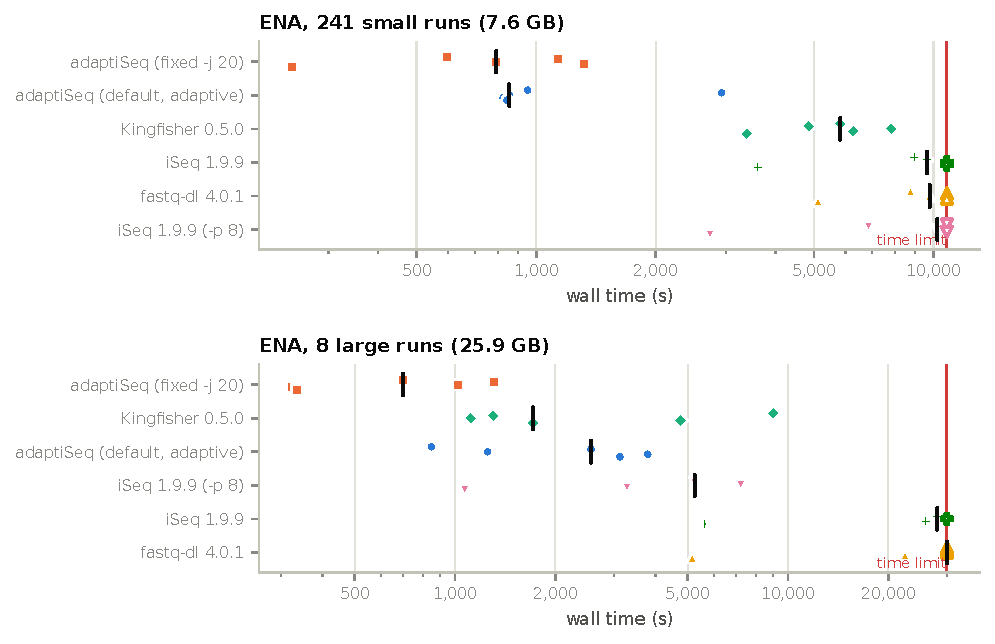
\includegraphics[width=\columnwidth]{figs/chain_wall.pdf}
\caption{Wall time of every arm in five repetitions on SDSC Expanse (build 0.1.12, Oct 26 to Nov 1). Filled markers finished, hollow markers hit the time limit and are lower bounds; black bars are medians; arms are ordered by median.}\label{fig:chainwall}
\end{figure}

The speed comes from connections. adaptiSeq's default held a median of 15.6 (D1) and 21.7 (D2) open connections to ENA, iSeq and fastq-dl one, iSeq \texttt{-p 8} up to eight, and Kingfisher a median of 1.7 and 4.0. Because ENA serves each connection at a few MB/s (P1), connections translate almost directly into throughput. Fixing the number of files in flight from 1 to 64 shows it directly (Fig.~\ref{fig:jsweep}): time falls roughly in proportion up to eight files, and the best median setting was 15 times faster than one file at a time on D1 and 23 times faster on D2. No single fixed value was best on both lists in all repetitions.

\begin{figure}[t]
\centering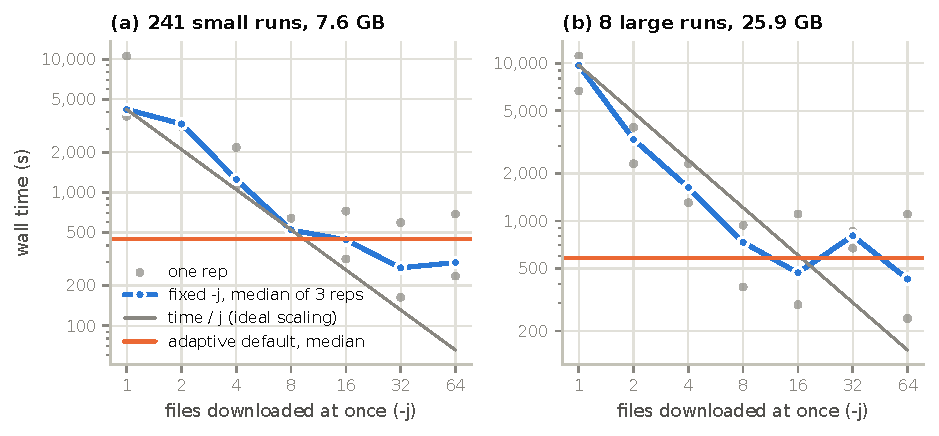
\includegraphics[width=\columnwidth]{figs/jsweep.pdf}
\caption{Wall time against the number of files in flight, fixed \texttt{-j} 1--64 (build 0.1.7, three repetitions; grey dots are single repetitions, blue the median, the grey line is perfect scaling, orange the adaptive default).}\label{fig:jsweep}
\end{figure}

\begin{table*}[t]
\caption{Final comparison, five repetitions per cell (build 0.1.12). Wall time and throughput are medians (arms marked $\dagger$ reached the time limit in at least three of five repetitions, so these are lower bounds on time); verified is the share of run downloads whose files all match ENA's MD5 (1,205 on D1, 40 on D2); short is the number of rows (of five) in which the arm exited 0 with fewer runs than requested.}\label{tab:chain}
\centering\small
\begin{tabular}{@{}l rrrr c rrrr@{}}
\toprule
& \multicolumn{4}{c}{D1: 241 runs, 7.6~GB} & & \multicolumn{4}{c}{D2: 8 runs, 25.9~GB}\\
\cmidrule{2-5}\cmidrule{7-10}
Arm & Wall (s) & MB/s & Verified & Short & & Wall (s) & MB/s & Verified & Short\\
\midrule
adaptiSeq, fixed \texttt{-j 20} & 794 & 9.54 & 99.8\% & 0 & & 699 & 37.0 & 100\% & 0\\
adaptiSeq, default & 855 & 8.87 & 99.8\% & 0 & & 2,561 & 10.1 & 100\% & 0\\
Kingfisher 0.5.0 & 5,825 & 1.29 & 85.1\% & 3 & & 1,715 & 5.44 & 57.5\% & 1\\
iSeq 1.9.9 & 9,628 & 0.77 & 78.5\% & 2 & & 28,053$^\dagger$ & 0.91 & 90.0\% & 0\\
iSeq 1.9.9 \texttt{-p 8} & 10,223$^\dagger$ & 0.74 & 81.1\% & 0 & & 5,245 & 4.89 & 97.5\% & 0\\
fastq-dl 4.0.1 & 9,778 & 0.78 & 66.6\% & 1 & & 30,000$^\dagger$ & 0.60 & 75.0\% & 1\\
\bottomrule
\end{tabular}
\end{table*}

\subsection{Completeness and honest failure}
Over the five repetitions adaptiSeq delivered 1,203 of 1,205 small-run downloads and 40 of 40 large-run downloads with every file verified (Table~\ref{tab:chain}, Fig.~\ref{fig:complete}); it delivered all runs in 16 of its 20 rows. In the other four, one run of D1 was missing: ENA's copy of a file failed MD5 three times or could not be opened, adaptiSeq exited 1 and named the run in \texttt{fail.log}. It never delivered a file it could not check against ENA (0 runs) and never exited 0 with a run missing (0 of 20 rows). The other tools exited 0 with runs short in 8 of their 40 rows and delivered 204 run downloads as files that cannot be checked against ENA's MD5, almost all because ENA's API answered without the FASTQ columns and the tool fetched the run from SRA instead (Kingfisher: 95 runs in one repetition; iSeq: 44). They also reached the time limit 10 times. For a user, the difference is whether the exit status can be trusted.

\begin{figure}[t]
\centering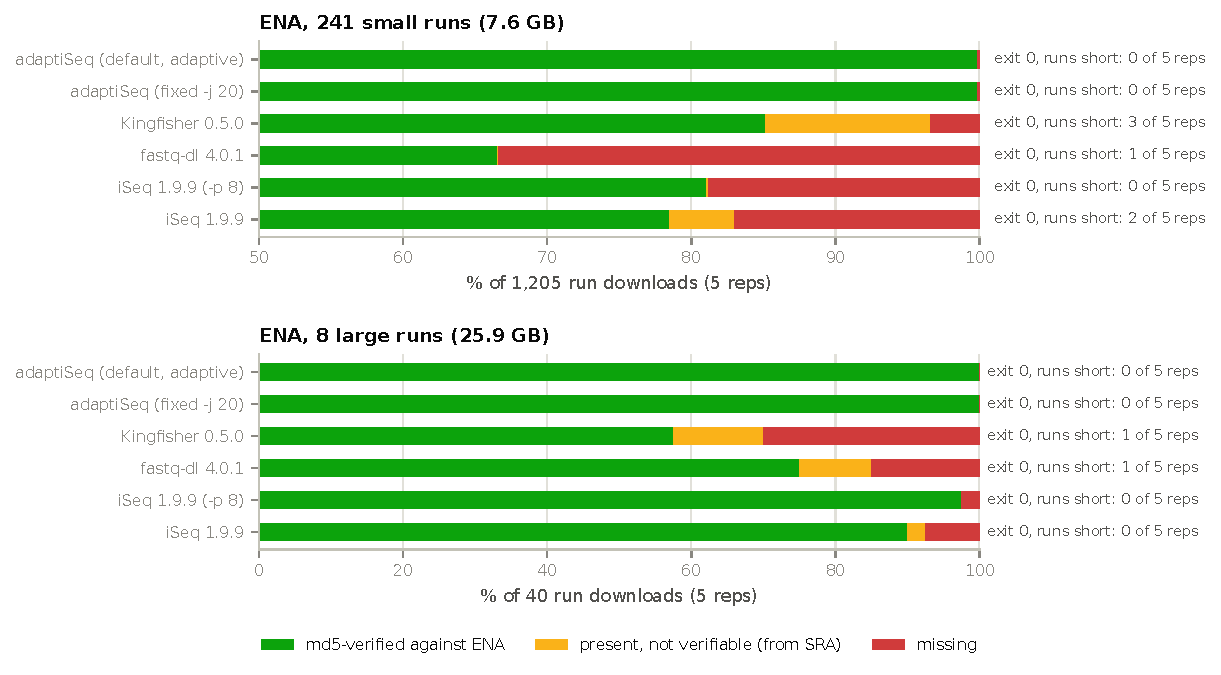
\includegraphics[width=\columnwidth]{figs/chain_complete.pdf}
\caption{Run downloads over five repetitions (1,205 on D1, 40 on D2), split into MD5-verified, present but not verifiable against ENA, and missing (including runs not reached before a time limit). Right: repetitions in which the arm exited 0 although runs were short. The D1 axis starts at 50\%.}\label{fig:complete}
\end{figure}

\subsection{Keeping connections busy, and verifying in the pool}
Fig.~\ref{fig:tail} shows archive connections over time for four runs of D2. In build 0.1.4 the batch moved most of the 26~GB in the first 25--35 minutes on 18--25 connections, then spent one to two and a half hours on one to three: the tail of each file on one range, and the serial per-run re-download of corrupt files. In 0.1.12 the same list held 25 connections until the last minutes and finished in 850 and 1,253~s. Across builds the median adaptive-default time on D2 fell from 6,552~s (0.1.4) to 2,561~s (0.1.12), and each step lines up with one mechanism: in-pool verification and the ceiling rule, work stealing, a retried range probe (an unanswered probe had been read as ``no range support'', sending 1.5--2~GB files down one connection) and cap recovery by time.

Corrupt copies hit every tool (P3). What differs is the consequence. adaptiSeq deleted each bad copy and fetched it again inside the pool, and verified every run of D2 in all ten of its final rows. iSeq's first retry re-checks the same file, so its three tries are two downloads; in one repetition both iSeq arms gave up on a D2 run after three tries. Kingfisher aborted a whole list on the first corrupt file in our first campaign.

\begin{figure}[t]
\centering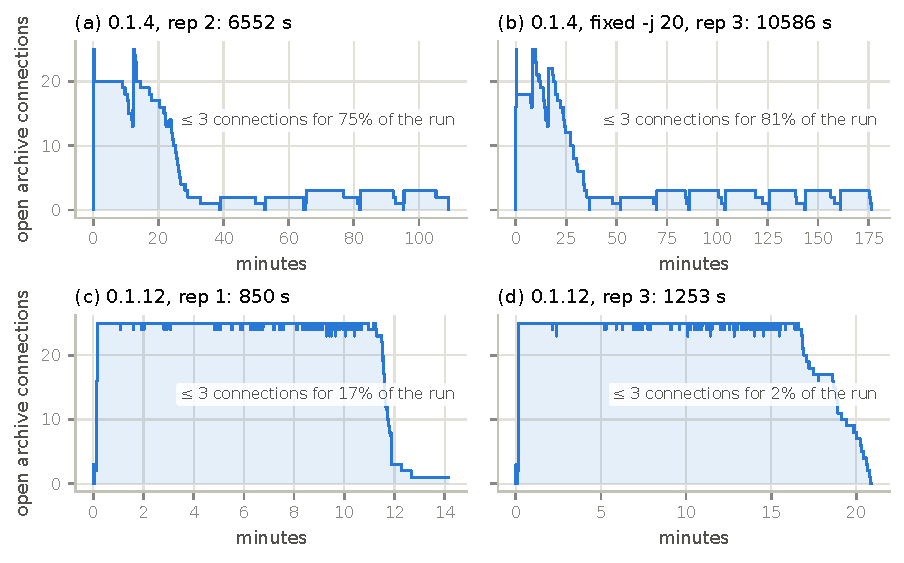
\includegraphics[width=\columnwidth]{figs/tail.pdf}
\caption{Open archive connections during four downloads of D2. (a, b) Build 0.1.4: after the batch the run sat on 1--3 connections for most of its length. (c, d) Build 0.1.12: 25 connections (ENA's ceiling that day) until the end.}\label{fig:tail}
\end{figure}

\subsection{Controllers across archives}\label{sec:ctrl}
Round 3 ran the five controllers and fixed pools of 20 and 64 on six lists from ENA, NCBI and GSA, three repetitions each (18 cases). No arm won everywhere: every arm was fastest in at least one case and over 1.5 times the fastest in another. By mean ratio to the fastest arm, fixed \texttt{-j 64} (1.35) was best, followed by topdown (1.39; worst case 3.80, an ENA slow spell that timed out four controllers alike), greedy (1.41), fixed \texttt{-j 20} (1.55), bottomup (1.62), budget (1.84) and knee (2.15). The two controllers that use the fewest connections (knee 12.8 and budget 13.1 on average, against 18.9 for topdown) were the slowest, and budget remains available for users who want to load the archive less. Topdown was chosen as the default for its average and worst case among the adaptive options.

\subsection{Where adaptation does not win}
The adaptive default was not the fastest setting. In the final comparison the fixed pool of 20 beat it in 9 of 10 panel-repetitions; the median ratio of default to fixed was 1.6 on D1 and 2.0 on D2. Three causes stand out in the logs. (i) A failed transport probe: in two repetitions the default's single HTTPS probe failed at the start, and the cached verdict sent the whole list to segmented FTP, which ENA resets under load; the default ran at 3.1 and 1.7 mean connections while the fixed pool used HTTPS at 15--20. This is a transport decision, not a controller decision; re-probing after failures is the obvious fix. (ii) Range refusals: in one repetition ENA answered 178 range requests with 403 and 29 with 416 during the default's run, which took 3,789~s while the fixed pool took 323~s a few hours later. (iii) A limit below the controller: in one repetition the default held about three connections for ten minutes while the controller held 20 workers, after ENA answered 20 single-connection requests with 403. Even so, the default needs no value chosen for the list, and on the controller panels its average was within 3\% of the best fixed pool; on NCBI extra connections bought nothing, and on GSA the best fixed value changed between repetitions. The fixed pool's advantage is specific to ENA's present behaviour, where more connections up to the ceiling nearly always help.

\section{Limitations}
All benchmark results come from one site, Expanse; per-connection rates elsewhere differ (a different site we probed saw 1.0--1.2~MB/s per ENA connection, within Expanse's range), though the per-connection behaviour was the same. The largest source of variance is the archive: paired ratios, repeated runs over days and reporting every repetition reduce but do not remove it, and a different week could reorder close arms. Arms in a repetition ran hours apart on D2 (single-connection tools take up to eight hours), so pairing shares the day, not the minute. The campaigns span builds 0.1.4 to 0.1.12; the tool comparison and the controller round each use one build, but cross-build comparisons mix design changes with archive changes. MD5 mismatch counts come from log lines whose wording differs between tools, and connections are sampled at 5~Hz and miss very short-lived ones. Time limits make the slow tools' times lower bounds, so their true ratios are larger than shown. The comparison concerns accession lists: for a single large file, a multi-connection downloader such as aria2c is likely as fast. Five repetitions give wide intervals. adaptiSeq is distributed through PyPI and not yet Bioconda and relies on external programs (\texttt{wget}; sra-tools and \texttt{pigz} when conversion is needed).

\section{Conclusion}
Downloading public sequencing data is limited by the archive, not the client's link: ENA serves each connection at a few MB/s, its API fails for hours, it serves corrupt copies, and it refuses connections past a moving ceiling. adaptiSeq answers each of these with many connections across and within files, kept busy to the last byte; refusals read as a ceiling; every file checked as it lands and re-fetched in parallel; and no silent substitution or skipping. On two ENA lists it was several times faster than iSeq, Kingfisher and fastq-dl in most repetitions, and it was the only tool whose exit status always matched what it delivered. Its adaptive default is a reasonable no-tuning setting rather than the fastest one. Source, accession lists, manifests, scripts and result tables are at \url{https://github.com/swargo98/adaptiSeq}; the package is at \url{https://pypi.org/project/adaptiseq/}.

\section*{Acknowledgments}
adaptiSeq is derived from iSeq~\cite{iseq} and its transfer engine from FastBioDL~\cite{fastbiodl}. This work used Expanse at the San Diego Supercomputer Center~\cite{expanse} through allocation CIS250262 from the Advanced Cyberinfrastructure Coordination Ecosystem: Services \& Support (ACCESS) program~\cite{access}, supported by U.S. National Science Foundation grants \#2138259, \#2138286, \#2138307, \#2137603 and \#2138296.

\begin{thebibliography}{99}
\bibitem{sra} K. Katz, O. Shutov, R. Lapoint, M. Kimelman, J. R. Brister and C. O'Sullivan, ``The Sequence Read Archive: a decade more of explosive growth,'' \emph{Nucleic Acids Res.}, vol. 50, pp. D387--D390, 2022.
\bibitem{ena} D. Yuan \emph{et al.}, ``The European Nucleotide Archive in 2025,'' \emph{Nucleic Acids Res.}, vol. 54, pp. D120--D127, 2026.
\bibitem{ddbj} T. Ara \emph{et al.}, ``DDBJ update in 2025: system integration for global data-sharing including pathogen surveillance,'' \emph{Nucleic Acids Res.}, vol. 54, pp. D106--D110, 2026.
\bibitem{gsa} T. Chen \emph{et al.}, ``The Genome Sequence Archive Family: toward explosive data growth and diverse data types,'' \emph{Genomics Proteomics Bioinformatics}, vol. 19, pp. 578--583, 2021.
\bibitem{iseq} H. Chao, Z. Li, D. Chen and M. Chen, ``iSeq: an integrated tool to fetch public sequencing data,'' \emph{Bioinformatics}, vol. 40, no. 11, btae641, 2024.
\bibitem{kingfisher} B. J. Woodcroft \emph{et al.}, ``Kingfisher: a utility for procurement of public sequencing data,'' Zenodo, 2024, doi:10.5281/zenodo.10525085.
\bibitem{fastqdl} R. A. Petit III \emph{et al.}, ``fastq-dl: efficiently download FASTQ files from SRA or ENA repositories,'' v4.0.1, Zenodo, 2026, doi:10.5281/zenodo.8051230.
\bibitem{fetchngs} H. Patel \emph{et al.}, ``nf-core/fetchngs v1.13.0,'' Zenodo, 2026, doi:10.5281/zenodo.22764959.
\bibitem{nfcore} P. A. Ewels \emph{et al.}, ``The nf-core framework for community-curated bioinformatics pipelines,'' \emph{Nat. Biotechnol.}, vol. 38, pp. 276--278, 2020.
\bibitem{pysradb} S. Choudhary, ``pysradb: a Python package to query next-generation sequencing metadata and data from NCBI Sequence Read Archive,'' \emph{F1000Research}, vol. 8, p. 532, 2019.
\bibitem{fastbiodl} R. M. Swargo, E. Arslan and M. Arifuzzaman, ``Adaptive parallel downloader for large genomic datasets,'' arXiv:2508.05511, 2025.
\bibitem{expanse} S. Strande \emph{et al.}, ``Expanse: computing without boundaries,'' in \emph{Proc. PEARC '21}, 2021, pp. 1--4.
\bibitem{access} T. J. Boerner, S. Deems, T. R. Furlani, S. L. Knuth and J. Towns, ``ACCESS: advancing innovation,'' in \emph{Proc. PEARC '23}, 2023, pp. 173--176.
\end{thebibliography}
\end{document}
